\documentclass[12pt,a4paper,fleqn]{article}
\title{Progress Report}
\author{Syed Ahmad Raza}
\date{2018.03.07}
\usepackage{mathtools}
\usepackage{graphicx}
\usepackage{color}          % for color eps output
% \usepackage{afterpage}
\usepackage{float}          % to force a figure placement with [H] command
\usepackage{enumitem}
\usepackage{newtxtext}
\usepackage{newtxmath}
\usepackage{nicefrac}
%\usepackage{layouts}       % for: \printinunitsof{in}\prntlen{\textwidth}

\begin{document}
\maketitle
%\tableofcontents
\pagebreak

\section{Solution of Navier-Stokes equations using\\
    Finite Volume Method for nonuniform grid}

\subsection{Discretization of the convective and diffusive terms for 2D nonuniform grid}

\begin{figure}[H]
    \centering
    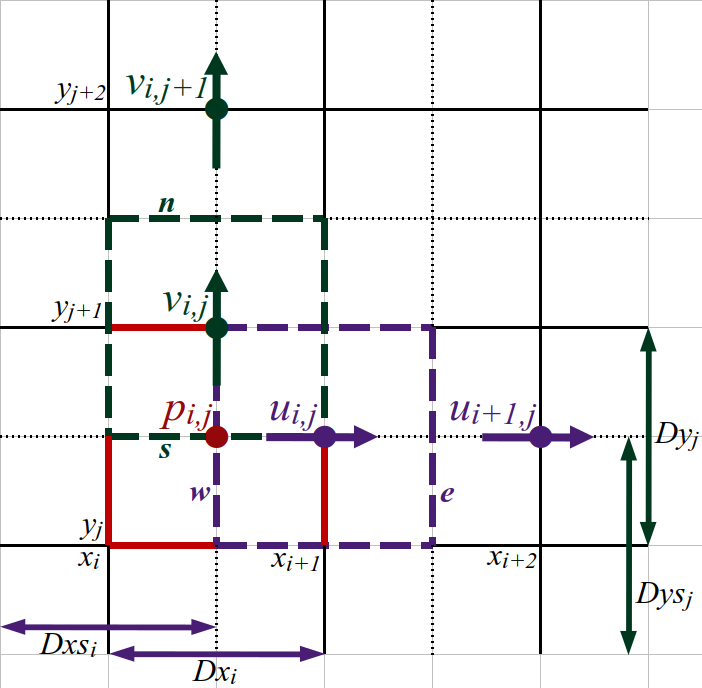
\includegraphics[width=0.5\textwidth]{staggered_grid.png}
    \caption{Visual representation of the staggered grid used for discretization in Finite Volume Method}
    \label{fig:staggered-grid}
\end{figure}

Linear interpolation is used for the velocities \(u_n, u_s, v_e,\) and \(v_w\). Let us analyze one of the velocities \(u_n\).

\begin{equation*}
\frac{u_n - u_{i,j}}{y_{j+1} - y_{j+\nicefrac{1}{2}}}
= \frac{u_{i,j+1} - u_{i,j}}{y_{j+\nicefrac{3}{2}} - y_{j+\nicefrac{1}{2}}}
\end{equation*}
\begin{equation*}
\frac{u_n - u_{i,j}}{\nicefrac{Dy_j}{2}}
= \frac{u_{i,j+1} - u_{i,j}}
{\left(\nicefrac{Dy_{j+1}}{2}\right) + \left(\nicefrac{Dy_j}{2}\right)}
\end{equation*}
\begin{equation*}
\frac{u_n - u_{i,j}}{\nicefrac{Dy_j}{2}}
= \frac{u_{i,j+1} - u_{i,j}}
{\nicefrac{\left(Dy_{j+1} +Dy_j\right)}{2}}
\end{equation*}

Therefore, the terms reduce to the following:
\begin{equation*}
\begin{aligned}
u_n &= u_{i,j} + \left(\frac{u_{i,j+1} - u_{i,j}}{Dys_{j+1}}\right)
\left(\frac{Dy_j}{2}\right)\\
u_s &= u_{i,j-1} + \left(\frac{u_{i,j} - u_{i,j-1}}{Dys_j}\right)
\left(\frac{Dy_{j-1}}{2}\right)
\end{aligned}
\qquad
\begin{aligned}
v_e &= v_{i,j} + \left(\frac{v_{i+1,j} - v_{i,j}}{Dxs_{i+1}}\right)
\left(\frac{Dx_i}{2}\right)\\
v_w &= v_{i-1,j} + \left(\frac{v_{i,j} - v_{i-1,j}}{Dxs_i}\right)
\left(\frac{Dx_{i-1}}{2}\right)
\end{aligned}
\end{equation*}

\subsubsection{Upwind scheme for velocities in the convective terms}
For rest of the velocities in convective terms, the upwind scheme may be used. For positive velocities,
\begin{equation*}
\begin{aligned}
u_e &= u_{i,j}\\
v_n &= v_{i,j}
\end{aligned}
\qquad\qquad
\begin{aligned}
u_w &= u_{i-1,j}\\
v_s &= v_{i,j-1}
\end{aligned}
\qquad\qquad
\begin{aligned}
u_{e,v} &= u_{i,j}\\
v_{n,u} &= v_{i,j}
\end{aligned}
\qquad\qquad
\begin{aligned}
u_{w,v} &= u_{i-1,j}\\ 
v_{s,u} &= v_{i,j-1}
\end{aligned}
\end{equation*}
For negative velocities,
\begin{equation*}
\begin{aligned}
u_e &= u_{i+1,j}\\
v_n &= v_{i,j+1}
\end{aligned}
\qquad\qquad
\begin{aligned}
u_w &= u_{i,j}\\
v_s &= v_{i,j}
\end{aligned}
\qquad\qquad
\begin{aligned}
u_{e,v} &= u_{i,j+1}\\
v_{n,u} &= v_{i+1,j}
\end{aligned}
\qquad\qquad
\begin{aligned}
u_{w,v} &= u_{i-1,j+1}\\ 
v_{s,u} &= v_{i+1,j-1}
\end{aligned}
\end{equation*}

For the first time step, Euler scheme is used and for subsequent time steps, Adams-Bashforth scheme is utilized.

\subsubsection{QUICK scheme for velocities in the convective terms}
QUICK scheme is also incorporated in the code, with an option to switch between upwind (first order) or QUICK scheme (second order). For positive velocities,
\begin{equation*}
u_e = \frac{u_{i} + u_{i+1}}{2} - \frac{Dx_{i+1}^2}{8Dxs_{i+1}}
\left(\frac{u_{i+1} - u_{i}}{Dx_{i+1}} - \frac{u_{i} - u_{i-1}}{Dx_{i}}\right)
\end{equation*}
\begin{equation*}
u_w = \frac{u_{i-1} + u_{i}}{2} - \frac{Dx_{i}^2}{8Dxs_{i}}
\left(\frac{u_{i} - u_{i-1}}{Dx_{i}} - \frac{u_{i-1} - u_{i-2}}{Dx_{i-1}}\right)
\end{equation*}
\begin{equation*}
v_n = \frac{v_{j} + v_{j+1}}{2} - \frac{Dy_{j+1}^2}{8Dys_{j+1}}
\left(\frac{v_{j+1} - v_{j}}{Dy_{j+1}} - \frac{v_{j} - v_{j-1}}{Dy_{j}}\right)
\end{equation*}
\begin{equation*}
v_s = \frac{v_{j-1} + v_{j}}{2} - \frac{Dy_{j}^2}{8Dys_{j}}
\left(\frac{v_{j} - v_{j-1}}{Dy_{j}} - \frac{v_{j-1} - v_{j-2}}{Dy_{j-1}}\right)
\end{equation*}

For negative velocities,
\begin{equation*}
u_e = \frac{u_{i} + u_{i+1}}{2} - \frac{Dx_{i+1}^2}{8Dxs_{i+2}}
\left(\frac{u_{i+2} - u_{i+1}}{Dx_{i+2}} - \frac{u_{i+1} - u_{i}}{Dx_{i+1}}
\right)
\end{equation*}
\begin{equation*}
u_w = \frac{u_{i-1} + u_{i}}{2} - \frac{Dx_{i}^2}{8Dxs_{i+1}}
\left(\frac{u_{i+1} - u_{i}}{Dx_{i+1}} - \frac{u_{i} - u_{i-1}}{Dx_{i}}\right)
\end{equation*}
\begin{equation*}
v_e = \frac{v_{j} + v_{j+1}}{2} - \frac{Dy_{j+1}^2}{8Dys_{j+2}}
\left(\frac{v_{j+2} - v_{j+1}}{Dy_{j+2}} - \frac{v_{j+1} - v_{j}}{Dy_{j+1}}
\right)
\end{equation*}
\begin{equation*}
v_w = \frac{v_{j-1} + v_{j}}{2} - \frac{Dy_{j}^2}{8Dys_{j+1}}
\left(\frac{v_{j+1} - v_{j}}{Dy_{j+1}} - \frac{v_{j} - v_{j-1}}{Dy_{j}}\right)
\end{equation*}

\subsection{2D results for nonuniform grid with higher order scheme}

A nonuniform grid was selected for the \(y\)-direction to provide a greater number of cells in the middle of channel flow, as per the following equation:

\begin{equation}\label{eq:y_grid_nonuniform}
y_j = \frac{L}{2}\left[
\tan \left\lbrace
\pi \left(\frac{x_i}{2L} - \frac{1}{4}\right)\right\rbrace
+ 1 \right]
\end{equation}

The code was run with first order upwind scheme and then using second order QUICK scheme. The results for two grid sizes are shown in the figures below.

\begin{figure}[H]
    \centering
    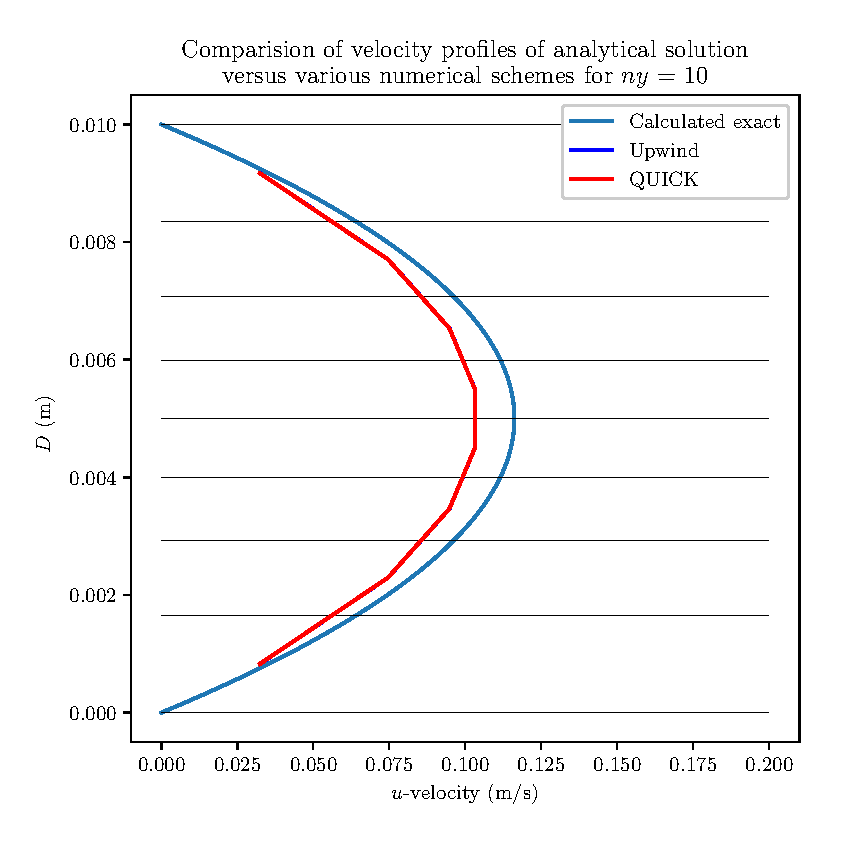
\includegraphics[width=\textwidth]{ny-10_profilesComparison.eps}
    \caption{Comparison of numerical results with analytical solution for nonuniform grid with two different schemes using y-direction grid intervals \(n_y = 10\).}
    \label{fig:ny-10_profilesComparison.eps}
\end{figure}

\begin{figure}[H]
    \centering
    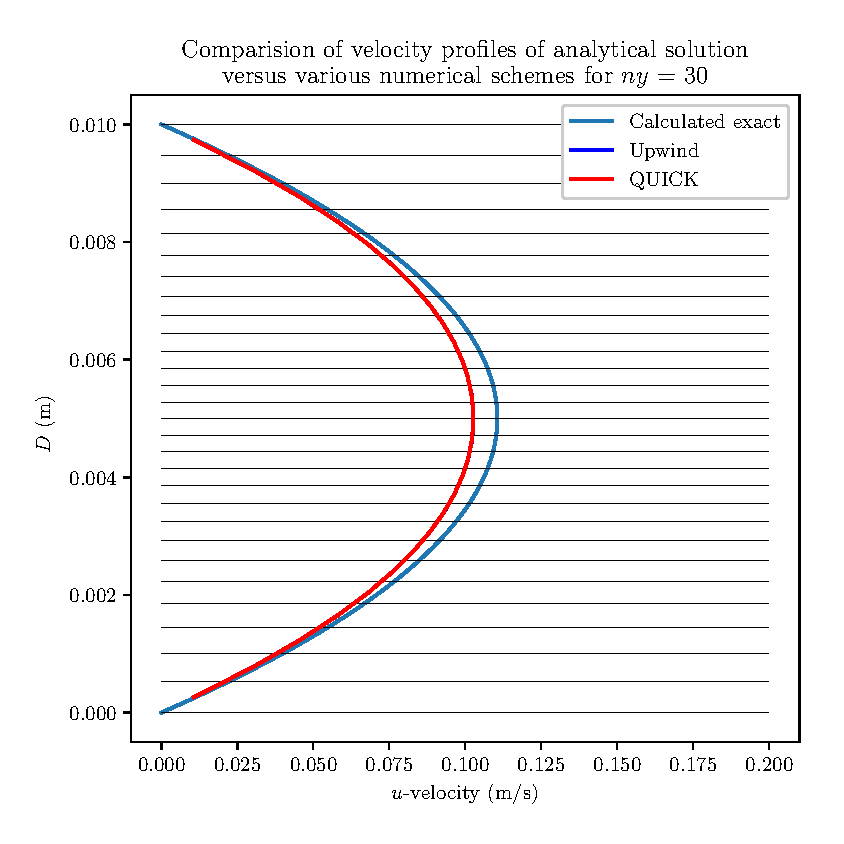
\includegraphics[width=\textwidth]{ny-30_profilesComparison.eps}
    \caption{Comparison of numerical results with analytical solution for nonuniform grid with two different schemes using y-direction grid intervals \(n_y = 30\).}
    \label{fig:ny-30_profilesComparison.eps}
\end{figure}
\newpage
\subsection{Discretization of the convective and diffusive terms for 3D nonuniform grid}
The convective and diffusive terms can be discretized using the individual components. To apply the projection method, the $u$-component equation can be written as
\begin{equation} \label{eq:3D-convective-diffusive-u}
\frac{\partial u}{\partial t} = -\frac{\partial uu}{\partial x} -\frac{\partial uv}{\partial y} -\frac{\partial uw}{\partial z} + \nu\left[\frac{\partial^2u}{\partial x^2} + \frac{\partial^2u}{\partial y^2} + \frac{\partial^2u}{\partial z^2}\right] \quad,
\end{equation}
which can be discretized as
\begin{align}\label{eq:3D-discretized_convective-diffusive-u}
\frac{\partial u}{\partial t} =
{}& - \frac{u_e^2 - u_w^2}{Dxs_{i+1}}
- \frac{u_n v_{n,u} - u_s v_{s,u}}{Dy_j}
- \frac{u_t w_{t,u} - u_b w_{b,u}}{Dz_k}
\nonumber\\
+ & \nu\left[
\left\{
\frac{u_{i+1,j,k}-u_{i,j,k}}{Dx_{i+1}}
- \frac{u_{i,j,k}-u_{i-1,j,k}}{Dx_i}
\right\}
\frac{1}{Dxs_{i+1}}
\right.\nonumber\\
& + \left\{
\frac{u_{i,j+1,k}-u_{i,j,k}}{Dys_{j+1}}
- \frac{u_{i,j,k}-u_{i,j-1,k}}{Dys_j}
\right\}
\frac{1}{Dy_j}\nonumber\\
& \left. + \left\{
\frac{u_{i,j,k+1}-u_{i,j,k}}{Dzs_{k+1}}
- \frac{u_{i,j,k}-u_{i,j,k-1}}{Dzs_k}
\right\}
\frac{1}{Dz_k}
\right] \quad .
\end{align}
where, for the \emph{diffusion terms}, second-order central scheme has been used. Similarly for the \(v\)- and \(w\)-components, the respective equations will be
\begin{equation} \label{eq:3D-convective-diffusive-v}
\frac{\partial v}{\partial t} = -\frac{\partial vu}{\partial x} -\frac{\partial vv}{\partial y} -\frac{\partial vw}{\partial z} + \nu\left[\frac{\partial^2v}{\partial x^2} + \frac{\partial^2v}{\partial y^2} + \frac{\partial^2v}{\partial z^2}\right]
\end{equation}
and 
\begin{equation} \label{eq:3D-convective-diffusive-w}
\frac{\partial w}{\partial t} = -\frac{\partial wu}{\partial x} -\frac{\partial wv}{\partial y} -\frac{\partial ww}{\partial z} + \nu\left[\frac{\partial^2w}{\partial x^2} + \frac{\partial^2w}{\partial y^2} + \frac{\partial^2w}{\partial z^2}\right] \quad,
\end{equation}
which can be discretized as
\begin{align}\label{eq:3D-discretized_convective-diffusive-v}
\frac{\partial v}{\partial t} =
{}& - \frac{v_e u_{e,v} - v_w u_{w,v}}{Dx_i}
- \frac{v_n^2 - v_s^2}{Dys_{j+1}}
- \frac{v_t w_{t,v} - v_b w_{b,v}}{Dz_k}\nonumber\\
+ & \nu\left[
\left\{
\frac{v_{i+1,j,k}-v_{i,j,k}}{Dxs_{i+1}}
- \frac{v_{i,j,k}-v_{i-1,j,k}}{Dxs_i}
\right\}
\frac{1}{Dx_i}
\right.\nonumber\\
& + \left\{
\frac{v_{i,j+1,k}-v_{i,j,k}}{Dy_{j+1}}
- \frac{v_{i,j,k}-v_{i,j-1,k}}{Dy_j}
\right\}
\frac{1}{Dys_{j+1}}\nonumber\\
& \left. + \left\{
\frac{v_{i,j,k+1}-v_{i,j,k}}{Dzs_{k+1}}
- \frac{v_{i,j,k}-v_{i,j,k-1}}{Dzs_k}
\right\}
\frac{1}{Dz_k}
\right] \quad ,
\end{align}
and
\begin{align}\label{eq:3D-discretized_convective-diffusive-w}
\frac{\partial w}{\partial t} =
{}& - \frac{w_e u_{e,w} - w_w u_{w,w}}{Dx_i}
- \frac{w_n v_{n,w} - w_s v_{s,w}}{Dy_j}
- \frac{w_t^2 - w_b^2}{Dzs_{k+1}}\nonumber\\
+ & \nu\left[
\left\{
\frac{w_{i+1,j,k}-w_{i,j,k}}{Dxs_{i+1}}
- \frac{w_{i,j,k}-w_{i-1,j,k}}{Dxs_i}
\right\}
\frac{1}{Dx_i}
\right.\nonumber\\
& + \left\{
\frac{w_{i,j+1,k}-w_{i,j,k}}{Dys_{j+1}}
- \frac{w_{i,j,k}-w_{i,j-1,k}}{Dys_j}
\right\}
\frac{1}{Dy_j}\nonumber\\
& \left. + \left\{
\frac{w_{i,j,k+1}-w_{i,j,k}}{Dz_{k+1}}
- \frac{w_{i,j,k}-w_{i,j,k-1}}{Dz_k}
\right\}
\frac{1}{Dzs_{k+1}}
\right] \quad .
\end{align}

%\subsection{Poisson equation of pressure}
%
%The Poisson equation for pressure can be written as
%\begin{equation} \label{eq:poisson-components}
%\frac{\partial^2 p}{\partial x^2}
%+ \frac{\partial^2 p}{\partial y^2}
%+ \frac{\partial^2 p}{\partial z^2}
%= \frac{\rho}{\Delta t} \left(
%\frac{\partial u^*}{\partial x}
%+ \frac{\partial v^*}{\partial y}
%+ \frac{\partial w^*}{\partial z}
%\right) \quad .
%\end{equation}
%Integrating it twice, discretizing and rearranging leads to
%\begin{align}
%p_{i,j}^{n+1} =
%&\frac{\rho}{\left[ - \frac{Dy_j}{Dxs_{i+1}} - \frac{Dy_j}{Dxs_i} - \frac{Dx_i}{Dys_{j+1}} - \frac{Dx_i}{Dys_j} \right]}
%\nonumber \\
%&\times
%\left[
%- \frac{Dy_j}{Dxs_{i+1}}p_{i+1,j} - \frac{Dy_j}{Dxs_i}p_{i-1,j} - \frac{Dx_i}{Dys_{j+1}}p_{i,j+1} - \frac{Dx_i}{Dys_j}p_{i,j-1}
%\right. \nonumber \\
%&\left.
%+ \frac{1}{\Delta t}\left\{
%\left(u^*_{i,j}-u^*_{i-1,j}\right)Dy_j
%+ \left(v^*_{i,j}-v^*_{i,j-1}\right)Dx_i
%\right\}
%\right]
%\quad .
%\end{align}
%This equation is employed using successive over-relaxation method (SOR).

\subsection{Poisson equation of pressure}
The Poisson equation of pressure in 3D may be written as
\begin{equation} \label{eq:3D-poisson-components}
\frac{\partial^2 p}{\partial x^2} + \frac{\partial^2 p}{\partial y^2} + \frac{\partial^2 p}{\partial z^2}
= \frac{1}{\Delta t} \left(\frac{\partial u^*}{\partial x} + \frac{\partial v^*}{\partial y} + \frac{\partial w^*}{\partial z}\right) \quad.
\end{equation}
Pressure may be found from the following discretized equation,
\begin{align}
p_{i,j,k}^{n+1} =
&\frac{1}{\left[ - \frac{Dy}{Dx1} - \frac{Dy}{Dx2} - \frac{Dy}{Dz1}- \frac{Dy}{Dz2} - \frac{Dx}{Dy1} - \frac{Dx}{Dy2} - \frac{Dx}{Dz1} - \frac{Dx}{Dz2} - \frac{Dz}{Dx1} - \frac{Dz}{Dx2} - \frac{Dz}{Dy1} - \frac{Dz}{Dy2}\right]}
\nonumber \\
&\times
\left[
- \frac{Dz}{Dx1}p_{i+1,j,k} - \frac{Dz}{Dx2}p_{i-1,j,k} - \frac{Dz}{Dy1}p_{i,j+1,k} - \frac{Dz}{Dy2}p_{i,j-1,k} \right.
\nonumber \\
&- \frac{Dy}{Dx1}p_{i+1,j,k} - \frac{Dy}{Dx2}p_{i-1,j,k} - \frac{Dy}{Dz1}p_{i,j,k+1} - \frac{Dy}{Dz2}p_{i,j,k-1}
\nonumber \\
&- \frac{Dx}{Dy1}p_{i,j+1,k} - \frac{Dx}{Dy2}p_{i,j-1,k} - \frac{Dx}{Dz1}p_{i,j,k+1} - \frac{Dx}{Dz2}p_{i,j,k-1}
\nonumber \\
&\left.
+ \frac{1}{\Delta t}\left\{
\left(u^*_{i,j,k}-u^*_{i-1,j,k}\right) \Delta y \Delta z
+ \left(v^*_{i,j,k}-v^*_{i,j-1,k}\right) \Delta x \Delta z
+ \left(w^*_{i,j,k}-w^*_{i,j,k-1}\right) \Delta x \Delta y
\right\}
\right]
\quad .
\end{align}


\subsection{Future work}
\begin{itemize}
\item Generate figures for 3D grid
\item Apply grid average and nodal value in QUICK scheme
\item Use Smagorinsky-Lilly turbulent model for 2D case
\end{itemize}

\end{document}
